\chapter{Dagens situasjon} \label{bakgrunn}
 Dette kapittelet vil ta for seg dagens situasjon og problemområde, deriblant bakgrunn for tap av sau på utmarksbeite, hvilke myndigheter som er involvert i prosessen med sanking og registrering av sau, hvilke krav som blir stilt for å ha sauer på utmarksbeite og hvordan slike oppsynsturer gjennomføres i dag. 

\section{Tap av sau}
Rundt to millioner sauer slippes på utmarksbeite i sommerhalvåret hvert år \cite[~s.1]{HansenTap2015} \cite{DyrebeskyttelsenNorgeTapBeite}. Dette er ikke uten risiko, for omlag 3-7\% av sauene mister livet som følge av sykdom, ulykker eller rovdyr hvert år \cite[~s.45]{Mattilsynet2019Arsrapport2019}. Dersom bøndene kan dokumentere at skadde eller døde sauer er forårsaket av fredet rovvilt, kan de søke om erstatning fra myndighetene for å dekke tapene \cite{2014ForskriftRovvilt, MiljdirektoratetErstatningRovvilt}. I 2020 var det rundt 15 000 sauer og lam som ble erklært drept og førte til erstatning \cite{Miljdirektoratet2020TapFr}. Resten av dødsfallene regnes som normaltap \cite{2014ForskriftRovvilt}. Trolig er det enda flere tap som aldri blir registrert ettersom kadaver på beite raskt råtner og fjernes av åtseletere \cite{Bakke2006TapRovdyr}. Ukentlige oppsynsturer er et av tiltakene for å forebygge tap og sikre dyrenes velferd samt stadfeste dødsårsak dersom et dyr har gått tapt. Sauebønder er lovpålagte å utføre disse ukentlige oppsynturene der de drar til utmarksbeitet og manuelt lokaliserer, sjekker og noterer ned dyrenes tilstand. Ved slutten av beitesesongen skal informasjonen om dyreflokken som er blitt innhentet gjennom oppsynsturene samles til en rapport som sendes til norske myndigheter. 

\subsection{Sykdom}
Ulike infeksjonsykdommer, feilernæring, parasittangrep og forgiftning er noen årsaker til sykdom blant småfe på utmarksbeite \cite{Johanssen2018AtferdSau}. Ved høy dyretetthet på beite og dårlig næringstilgang vil dyrene beite tettere opp mot sin egen avføring, og hvor det vil være høy forekomst av parasittlarver \cite{Tjrhom2019ForebyggingBeitebruk}. Særlig utsatt for parasittsykdom er kopplam, som er lam oppfostret på melk fra flaske og ikke direkte fra søye \cite{Tjrhom2019ForebyggingBeitebruk} siden de går glipp av den viktige råmelka som gjør dem motstandsdyktige for infeksjoner \cite[s.44]{engenForingAvKopplam2017}. Langs kysten av Sørvest-Norge er sykdommen alveld også en fare for lam \cite{Velle2018Alveld}. Lammene blir forgiftet og får leverskade av å konsumere planten rome \cite{Velle2018Alveld}, og det finnes ingen effektiv behandling mot selve alvelden foruten å prøve å forebygge det ved å unngå beiteområder med mye romeplante \cite{Sauehelsenett2017Alveld}. Ellers er god forsyning av råmelk til nyfødte lam, vaksiner, parasittbehandling, beiterotasjon, god fôring og jevnlig oppsyn på beite tiltak som forebygging av sykdom av småfe på beite \cite{Tjrhom2019ForebyggingBeitebruk, Johanssen2018AtferdSau}. 

\subsection{Ulykker}
Typiske ulykker som rammer småfe på beite er fallulykker, påkjørsler eller at dyrene blir sittende fast i beitelandskapet \cite{Dyrevernalliansen2019SauHusdyr}. Moderne saueraser er avlet for å gi mye kjøtt og ull, som resulterer i tyngre dyr. Dette gjør at dyrene lettere setter seg fast i myrer eller elver og ikke kommer seg løs, som fører til langstrakt lidelse og død \cite{Dyrevernalliansen2019SauHusdyr}. Det gjør dem også lettere bytter til rovvilt. Løshunder og rovvilt som jager dyrene kan også føre til at småfe får panikk og utsetter seg selv for fare som for eksempel å falle utenfor et stup eller bli drevet ut i vann.  

\subsection{Rovdyr} \label{sub:rovdyr}
Fredet rovvilt i Norge er bjørn, gaupe, jerv, ulv og kongeørn \cite{MiljdirektoratetRovbase}. Under særskilte tilfeller kan det også gis erstatning for husdyr tatt av havørn, som også er et fredet rovdyr \cite{2014ForskriftRovvilt}. Fordelingen av rovdyrenes andel av total tap av sau vises på figur \ref{fig:rovdyr_andel} under.

\begin{figure}[H] 
\centering
\captionsetup{width=.8\linewidth}
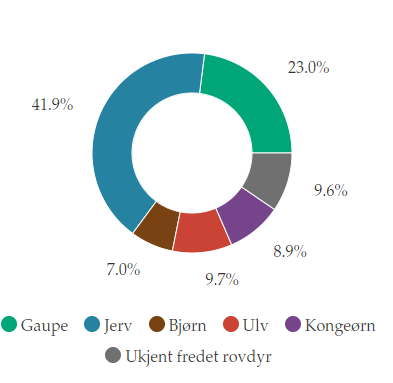
\includegraphics[]{Figurer/diagram/andel_rovvilt_diagram.png}
\caption{Fordeling av fredet rovvilts andel av total tap av sau}
\source{Rovbase \cite{RovbaseErstatningSau}}
\label{fig:rovdyr_andel}
\end{figure}

\noindent
Parallelt som det arbeides med sikre levedyktige rovviltbestander, er det også lagt ned stor innsats for å redusere tap av sau til rovvilt. Det har vist seg å gi en positiv effekt \cite{Klima-ogmiljdepartementet2020RekordlaveRovvilt}. Selv om antall innmeldte tap og påviste rovviltskader har blitt stadig færre, er det et ønske om å redusere tap av sau til rovvilt ytterligere \cite{Miljdirektoratet2020RekordlavtSau}. Dette gjelder særlig i Trøndelag, som er det fylket som stod for størst tap av sau til rovvilt i 2020 \cite{Miljdirektoratet2021Rovvilt2020}. Samme år ble det bevilget omlag 80 millioner kroner til tiltak som rovviltavvisende gjerder, beiteslipp og tidlig nedsanking \cite{Klima-ogmiljdepartementet2020RekordlaveRovvilt}. Andre tiltak som kan bidra til mer effektiv sanking av beitedyr samt bidra til å finne døde eller skadde dyr vil også bli støttes av statlige tilskudd \cite{Klima-ogmiljdepartementet2020RekordlaveRovvilt}. Kostnadene for å dekke erstatning av sau og lam til rovvilt var i 2020 på nærmere 38 millioner kroner \cite{Miljdirektoratet2021Rovvilt2020}. Effektivisering av oppsynsturer vil derfor ikke bare kunne forebygge lidelse blant småfe og gjøre prosessen for oppsyn enklere for bønder og beitelag, men også være økonomisk gunstig for både bønder og staten. 

\section{Involverte myndigheter}
Myndighetene som er involvert i oppfølging av sau på beite i Norge er per dags dato kommunen og Statsforvalteren som er relevant for det respektive beitelaget, samt Mattilsynet og Statens Naturoppsyn. I denne seksjonen skal deres ansvarsområde og informasjonsflyten mellom dem og bøndene beskrives. 

\subsection{Statsforvalteren}
Statsforvalteren (tidligere Fylkesmannen) har ansvar for å følge opp vedtak, mål og retningslinjer fra Stortinget og regjering, og har i tilegg en viktig rolle som bindeledd mellom stat og kommune \cite{Statsforvalteren202HistoriaStatsforvalteren}. I sammenheng med oppfølging av sau på beite, har Statsforvalteren ansvar for forvaltning av  \cite{Statsforvalteren2021Styringsdokumenter}: 
\begin{itemize}
    \item Produksjonstilskudd til beitelag.
    \item Tilskudd til spesielle miljøtiltak i jordbruket (SMIL) som fremmer natur-og kulturverdiene i jordbrukets kulturlandskap og redusere forurensningen fra jordbruket \cite{LandbruksdirektoratetTilskuddSMIL}.
    \item Erstatning for beitedyr tatt av rovvilt.
    \item Tilskudd til forebyggende og konflikt-dempende tiltak.
\end{itemize}

\subsection{Mattilsynet}
Mattilsynet er et statlig forvaltningsorgan med ansvar for å fremme blant annet dyrehelse og etisk forsvarlig hold av dyr \cite{Mattilsynet2021OmMattilsynet}. Dette arbeidet utføres ved å veilede om regelverk, formidle informasjon og føre risikobasert oppsyn for å forebygge dyrelidelser og utbrudd av smittsomme sykdommer \cite{Mattilsynet2021OmMattilsynet, Mattilsynet2021SauGeit}. Mattilsynet får tilsendt beitelagets rapport over oppsynsturene fra Statsforvalteren og gjennomfører en risikovurdering av dyrevelferden på utmarksbeite \cite{Mattilsynet2019TapRovvilt}, mer detaljer om risikoklassene er beskrevet i \ref{dyrevelferd}. Dersom Mattilsynet konkluderer med at dyreeier ikke tilfredsstiller kravene for god dyrevelferd, kan Mattilsynet kreve at dyreeier iverksetter risikoreduserende tiltak som deriblant økt oppsyn \cite{Mattilsynet2019TapRovvilt}. Retter ikke dyreholderen seg etter Mattilsynets pålegg vil Mattilsynet trappe opp bruken av virkemidler, som tvangsmulkt, overtredelsesgebyrer eller å gjennomføre tiltak på eierens regning \cite{Mattilsynet2019TapRovvilt}. I de mest alvorlige tilfellene kan Mattilsynet ta dyrene i midlertidig forvaring eller omplassere dem, avvikle dyreholdet, nekte den ansvarlige å drive aktiviteter som har med dyr å gjøre eller anmelde forholdet til politiet \cite[~s.4]{Mattilsynet2020Mattilsynets2020}. 

\subsection{Statens Naturoppsyn}
\acrfull{sno} er en avdeling i Miljødirektoratet og opererer som miljøforvaltningens operative feltorgan \cite{KjrstadStatensSNO}.
Hvis den oppsynsansvarlige finner et skadd eller dødt dyr og mistenker at det er et fredet rovvilt som står bak, må dyreeieren selv ta kontakt og vise kadaveret til \acrshort{sno} \cite[~s.18]{StatsforvaltereniInnlandet2020InformasjonInnlandet}. \acrshort{sno}s rovviltkontakter vil vurdere kadaveret og konkludere om skaden skyldes rovvilt eller ikke. Alle tap av husdyr erstattes fullt ut etter innsendt søknad hvis det er påvist at fredet rovvilt har forårsaket tapet \cite[~s.18]{StatsforvaltereniInnlandet2020InformasjonInnlandet}. Det gis også erstatning når det er sannsynlighetsovervekt for at tapet skyldes rovvilt \cite[~s.18]{StatsforvaltereniInnlandet2020InformasjonInnlandet}. For å komme frem til en konklusjon om tapet skyldes rovvilt, vil Statsforvalteren bruke opplysningene om beitelagets besetning og drift fra søknaden samt innhente kunnskap om rovviltbestandene og tapsforholdene i området fra kommune/landbrukskontoret og Mattilsynet \cite[~s.18]{StatsforvaltereniInnlandet2020InformasjonInnlandet}.

\begin{figure}[H]
\centering
\captionsetup{width=.8\linewidth}
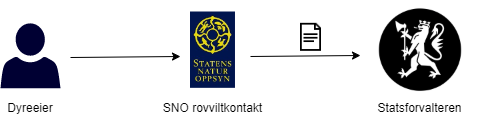
\includegraphics[width=0.9\linewidth]{Figurer/diagram/informasjonsflyt rovvilt.png}
\caption{Informasjonsflyt ved erstatning for sau drept av fredet rovvilt}
\label{fig:informasjonsflyt_rovvilt}
\end{figure}

\subsection{Informasjonsflyt ved innsending av oppsynturrapporter}
Dersom et beitelag ønsker å søke om tilskudd til produksjon og drift av beitelaget, må de lage en samlet rapport over alle oppsynsturene som er gjennomført over perioden der dyrene er på utmarksbeite med nødvendig informasjon \cite{Statsforvalteren2021Styringsdokumenter}. Med nødvendig informasjon menes opplysninger som antall døde og skadde dyr, funn eller observasjoner fra rovvilt, beiteforhold, kartinformasjon der observasjonen fant sted osv. Denne rapporten blir sendt til den aktuelle kommunen. \acrshort{nsg} har lagt ut et forslag til slik rapportskjema på deres nettsider, og dette skjemaet har blitt brukt som utgangspunkt for den innsendte rapporten til Stasforvalteren, se vedlegg \ref{rapportskjema}. Etter at kommunen har godkjent rapporten, blir den sendt videre til Statsforvalteren som har ansvaret for å forvalte produksjonstilskuddet og andre relevante tilskudd. Statsforvalteren videresender også oppsynsrapportene til Mattilsynet, som vil gjennomføre en risikovurdering av dyrenes velferd på beitet. Denne flyten er visualisert i figur \ref{fig:informasjonsflyt_rapport}.

\begin{figure}[H]
\centering
\captionsetup{width=.8\linewidth}
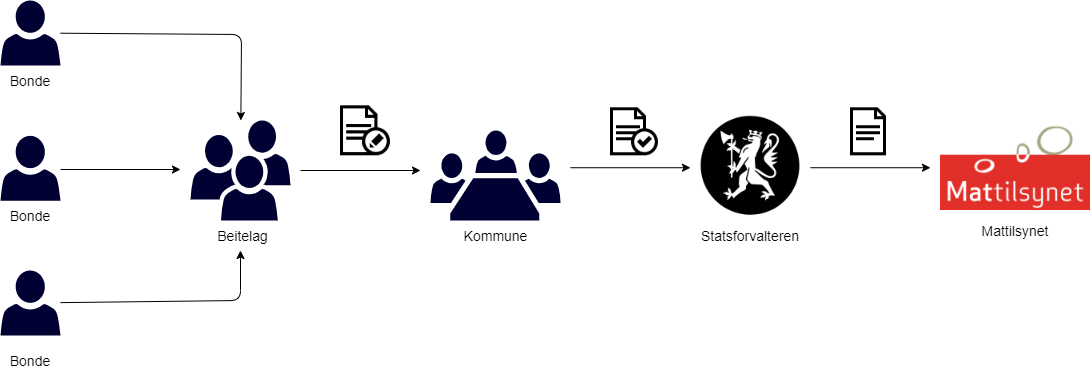
\includegraphics[width=0.9\linewidth]{Figurer/diagram/informasjonsflyt tilsynsrapport.png}
\caption{Informasjonsflyt mellom sauebønder og involverte myndigheter for innsending av oppsynsturrapporter}
\label{fig:informasjonsflyt_rapport}
\end{figure}

\section{Krav fra myndighetene}
\subsection{Oppfølging}
For å beskytte småfe fra unødig lidelse og død, er bønder lovpålagt å føre oppsyn av småfe på utmarksbeite minst én gang i uken \cite{2014ForskriftRovvilt}. I områder med kjent forekomst av rovvilt, må oppsynsfrekvensen være hyppigere enn én gang i uken \cite{2014ForskriftRovvilt}.

\subsection{Øremerking}
Småfe på beitet skal merkes med øremerker som er godkjent av Mattilsynet \cite{2005ForskriftSmafe}. Sau skal merkes med både elektronisk og visuelt merke 30 dager etter fødsel \cite{Mattilsynet2013remerkingSmafe}. Disse elektroniske øremerkene kan deretter leses av med en elektronisk håndleser for å lese av data \cite[~s.48]{BungerSmafenaring2018}. Følgende informasjon skal være med i øremerket for at dyret skal kunne identifiseres \cite{2005ForskriftSmafe}: 
\begin{itemize}
    \item Mattilsynet: MT.
    \item Nasjonalitetsidentifikasjon: NO.
    \item Dyreholdets spesielle identitetsnummer tildelt av Mattilsynet: 7 siffer.
    \item Individnummer: 5 siffer der første siffer er fødselsårets siste siffer og de følgende siffer er dyrets individ nummer.
\end{itemize}
Figuren under viser et eksempel på et øremerke for sau: 

\begin{figure}[H]
\centering
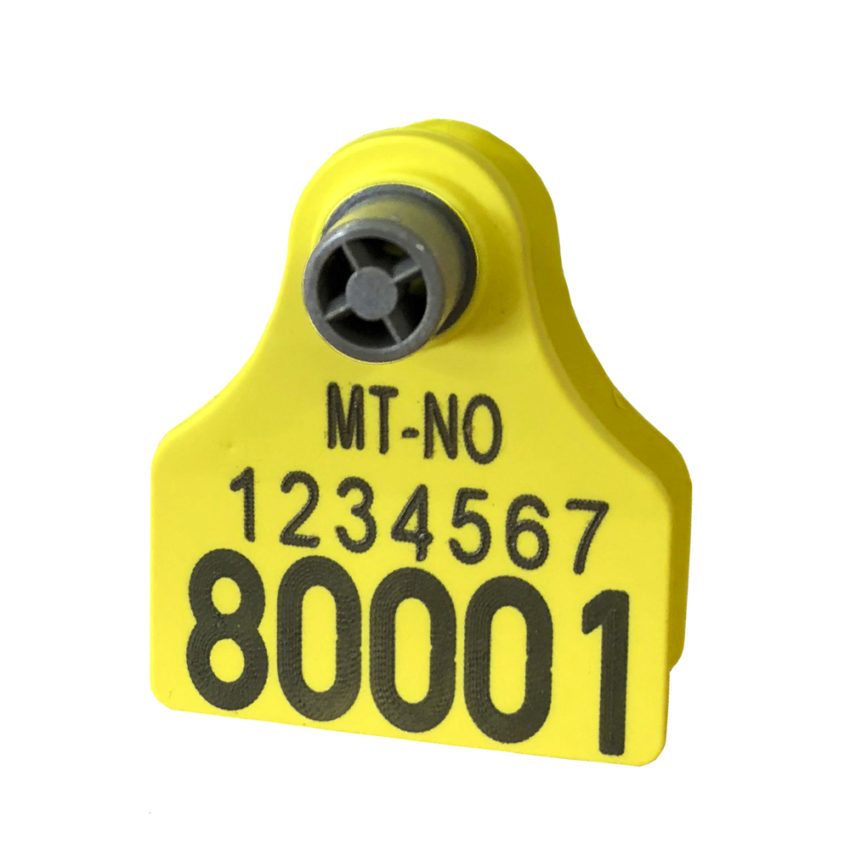
\includegraphics[scale=0.25]{Figurer/Bilder/oremerke.jpg}
\caption{Øremerke for sau}
\source{\cite{OSIDASCombiremerke}}
\label{fig:oremerke}
\end{figure}

\subsection{Dyrevelferd} \label{dyrevelferd}
For å sikre god helse og trivsel blant småfe samt sikre at det tas hensyn til dyrenes naturlige behov, er bønder lovpålagt å holde småfe på egnet utmarksbeite i minst 16 uker hvert år \cite{2005ForskriftSmafe}. Med utmarksbeite menes beite i naturlig vill vegetasjon, skog og fjellterreng som ikke blir kultivert eller gjødslet \cite[~s.55]{BungerSmafenaring2018}. Ansvaret for dyrenes velferd på utmarksbeite ligger hos dyreeier \cite{Mattilsynet2019TapRovvilt}. Mattilsynet vil sørge for at dyreholdet følges i henhold til dyrevelferdsloven; forskriften for velferd hos småfe og produksjonsdyr \cite{Mattilsynet2019TapRovvilt}. Dyreeier og gjetere på oppsynstur har meldeplikt dersom det oppdages smitteutbrudd, rovvilt eller andre årsaker til lidelse eller død blant dyrene på utmarksbeite. Mattilsynet opererer med tre risikoklasser for dyr på utmarksbeite \cite[~s.6]{Mattilsynet2019TapRovvilt}: 

\begin{itemize}
    \item \textbf{Lav risiko}
    \newline
    Tap av under 2\% for søyer, 6\% for lam og 4\% på besetningsnivå ligger innenfor det akseptable, men det forutsettes at det arbeides for å redusere totaltapet på sikt.
    \item \textbf{Middels risiko}
    \newline
    Tap mellom 2-6\% på søyer, 6-15\% på lam og mellom 4–10\% på besetningsnivå ligger innenfor et område hvor det forventes at forebyggende tiltak planlegges og gjennomføres.
    \item \textbf{Høy risiko}
    \newline
    Tap over 6\% på søyer, 15\% på lam og 10\% på besetningsnivå er i utgangspunktet uakseptabelt dyrevelferdsmessig sett. Forebyggende tiltak må planlegges og gjennomføres. 
\end{itemize}

\noindent
Mattilsynet vil vurdere risikonivået for hver enkelt beitelag ut i fra lokal kunnskap om beiteforholdene fra regionale representanter fra \acrlong{obb}, \acrfull{nibio} og søknadene for produksjonstilskudd og erstatning for tap av sau på beite \cite{Mattilsynet2019TapRovvilt}. Oversikt over estimert rovviltbestand og dokumenterte tap til rovvilt blir også hentet fra Rovbase \cite{Mattilsynet2019TapRovvilt}. 

\section{Gjennomføring av oppsyn}
I dag er det vanlig at flere bønder fra nærliggende områder går sammen og oppretter et beitelag der de samarbeider om oppsyn, sanking eller andre aktiviteter knyttet til utmarksbeite \cite[~s.57]{BungerSmafenaring2018}. I 2017 var ca. 74\% av all sau som ble sluppet på utmarksbeite inkludert i et organisert beitelag \cite{NorskSauogGeit2018OrganisertBeitebruk}. Beitelag er et av tiltakene i ordningen kalt \acrfull{obb} som ble opprettet i 1970 som et samarbeid mellom Landbruksdepartementet og \acrfull{nsg} \cite{NorskSauogGeit2018OrganisertBeitebruk}. Hovedmålsettingen for \acrshort{obb} er å legge til rette for en mer rasjonell utnytting av utmarksbeitene og redusere tapet av dyr på beite til et minimum \cite{NorskSauogGeit2018OrganisertBeitebruk}. I 2003 ble innført krav der beitelag må registreres i enhetsregisteret i Brønnøysund for å være berettiget tilskudd \cite{NorskSauogGeit2018OrganisertBeitebruk}.

\subsection{Før utslipp}
\acrshort{nsg} har kommet ut med en offisiell anbefaling om at søyer som skal slippes løs på utmarksbeite bør merkes med bjelleslips \cite{NorskSauogGeitBjelleslips}. Et bjelleslips er et merke som indikerer antall lam som er tilknyttet en søye med fargekoder, se figur \ref{fig:bjelleslips} under. Det gjør det mulig å for personer på oppsynsturer å få oversikt over dyretall på utmarksbeite. Det kan også lønne seg med bjelleslips dersom ens saueflokk blander seg med en annen besetning som ikke benytter seg av bjelleslips \cite[~s.27]{FylkesmanneniOsloogAkershus2017BeitedyrRovdyr}. 

\begin{figure}[H]
\centering
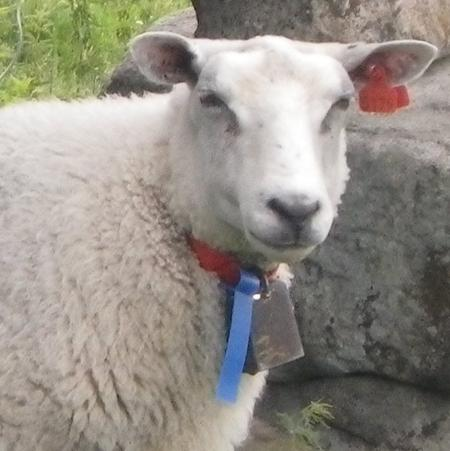
\includegraphics[scale=0.3]{Figurer/Bilder/bjelleslips.jpg}
\caption{Bjelleslips for sau}
\source{\cite{NorskSauogGeitBjelleslips}}
\label{fig:bjelleslips}
\end{figure}

\noindent
\acrshort{nsg} anbefaler å bruke samme fargekoding for slips som for fostertelling, som er når man undersøker antall fostre i en drektig søye med ultralyd \cite{FostertellingOgSniktitt2015}. Fargekodingen kan variere fra landsdel til landsdel. Masteroppgaven vil ta utgangspunkt i fargekodene som brukes i Oppdalområdet etter professor Hvasshovds erfaring med Søndre Trollheimen Beitelag som er følgende: 
\begin{itemize}
    \item Blått slips: 0 lam. 
    \item Grønt slips: 1 lam.
    \item Gult slips: 2 lam.
    \item Rødt slips: 3 lam. 
\end{itemize}
Det er ikke alle bønder som markerer at en søye ikke har lam og vil da bare unnlate å markere søyen med bjelleslips.

\subsection{På utmarksbeite}
Det er ikke en fastsatt dato for når småfe blir sluppet til utmarksbeite, men det skjer som oftest kort tid etter lammesesongen som forekommer rundt april og mai \cite{yrehagen2015BeiteUtmark}. Dyrevelferdsloven krever at samtlige dyr har god helsetilstand og at lam er sammen med mordyr og i stand til å holde følge med mora på beitet \cite{2005ForskriftSmafe}. Dyreeier må derfor selv vurdere hva som er best slippetidspunkt for sine dyr ut i fra deres alder og tilstand, og forholdene på beiteområdet \cite{NorskSauogGeitRiktigSlippetidspunkt}. Slipptidspunktet må være sent nok til det er nok beite som gir god nok næring slik at lammene får en jevn og god tilvekst, men tidlig nok til at søyene kan sortere ut de gode beiteplantene mens de er unge og næringsrike \cite[~s.8]{RekdalTemahefteSau}. Hvis beiteområde inneholder for eksempel høy vannføring i bekker, snøfonner o.l, må lammene være tilsvarende robuste \cite{NorskSauogGeitRiktigSlippetidspunkt}. 
\newline
\newline
Selve gjennomføringen av oppsynsturene vil naturlig nok variere fra bonde til bonde. Turene kan gjennomføres enten av den enkelte bonde eller gjennom organiserte beitelag. Heretter vil personer som utfører oppsynsturer bli referert til som oppsynsansvarlig. Per i dag utføres oppsynsturer ved at den oppsynsansvarlige, enten manuelt eller ved hjelp av digitale verktøy (eksempler på slike verktøy presenteres i kapt. \ref{sporing}), først sporer opp dyreflokken. Ettersom dyrene beveger seg raskt over store områder og gjerne i ulendt terreng, må den tilsynsansvarlige som regel observere dyrene på avstand med kikkert og deretter notere informasjon som antall og tilstand med penn og papir. Å registrere riktig antall kan fort bli en utfordring siden sauene gjerne beveger seg mens den tilsynsansvarlige ser vekk ifra kikkerten for å notere. De store avstandene fører også til at det kan være vanskelig å få øye på øremerker eller bjelleslips, selv med kikkert. I tillegg til antall sauer på beitet, vil dato, rute for oppsynstur og opplysninger som skadde dyr, årsak, observasjon av rovvilt og beiteforhold bli registrert. Ifølge professor Hvasshovds erfaring med tilsynsturer, pleier det å ta ca. 2-3 timer, men det kan ta opptil 10 timer dersom det er vanskelig å spore opp hele dyreflokken. 

\subsection{Sanking}
I følge \textit{Forskrift om velferd for småfe} \S 27 så har dyreeier ansvar for at småfe på utmarksbeite hentes hjem i god tid før det ventes frost eller snøfall om høsten \cite{2005ForskriftSmafe}. I følge data fra \acrlong{obb} pleier nedsankingen av sau å foregå i september \cite[~s.8]{Stornes2017TidligInnmarksbeite}. Tidlig innsanking av dyrene i august kan forekomme som et tiltak for å forebygge tap av småfe til rovvilt, da særlig jerv. Over 80 \% av skader på sau og lam utført av jerv blir påvist etter 1.august, og nesten halvparten av disse skjer etter 1.september \cite{Messel2016BondeMedisin}. Dersom en sauebonde velger å gjennomføre tidlig innsanking av dyrene, skal bonden bli kompensert for økningen av kostnadene for kraft -og grovfôr som følge av at dyrene må flyttes til innmarksbeite \cite[~s.10]{Stornes2017TidligInnmarksbeite}. Selve nedsanking av sau er utfordrende, ettersom det kan være vanskelig å finne hele dyreflokken og det er store områder å dekke. Hvis et beitelag har sluppet dyrene samlet, må dyrene også sorteres etter nedsankingen slik at dyrene drar til riktig bonde \cite{NorturaMedlem2016UtformingSA}. 

\section{Konklusjon}
Det er lovpålagt for norske sauebønder å slippe sau på utmarksbeite i minst 16 uker årlig. Hvert år mister 3-7\% av sauer sluppet på utmarksbeite livet grunnet sykdom, ulykker eller rovdyr. Selv om tallene på tap av sau på beite er i nedgående trend, arbeides det med å senke tapene ytterligere både for å minimere dyrenes lidelser samt de økonomiske tapene det forårsaker. Dette arbeides med både fra sauebøndene og beitelagenes side, og fra offisielle myndigheter som Statsforvalteren, Mattilsynet og Statens Naturoppsynet. Et av tiltakene for å redusere tap er å utføre ukentlige tilsynsturer der dyreflokkens antall og tilstand sjekkes, samt om det rovvilt tilstede i nærområdet. Oppsynet gjennomføres ved at den personen som er ansvarlig for tilsyn sporer opp dyreflokken og registrerer relevant informasjon som videresendes til Statsforvalteren og Mattilsynet, som vil vurdere om det er behov for ytterligere tiltak for å sikre velferden til dyrene eller gi erstatning for tapte dyr. 